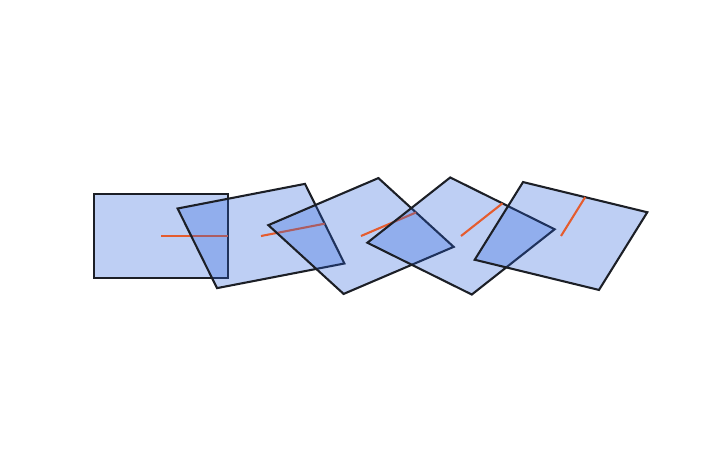
\begin{tikzpicture}[every node/.style={inner sep=0bp,outer sep=0bp}]
  \definecolor{qcA}{rgb}{0.16,0.38,0.86}
  \definecolor{qcB}{rgb}{0.11,0.12,0.15}
  \definecolor{qcC}{rgb}{0.9,0.36,0.18}
  \useasboundingbox (0bp,0bp) rectangle (240bp,150bp);
  \path[fill=qcA,fill opacity=0.3,draw=qcB,line width=0.75bp] (24bp,60bp) -- (72bp,60bp) -- (72bp,90bp) -- (24bp,90bp) -- cycle;
  \path[draw=qcC,line width=0.75bp] (48bp,75bp) -- (72bp,75bp);
  \path[fill=qcA,fill opacity=0.3,draw=qcB,line width=0.75bp] (68.164bp,56.237bp) -- (114.021bp,65.103bp) -- (99.836bp,93.763bp) -- (53.979bp,84.897bp) -- cycle;
  \path[draw=qcC,line width=0.75bp] (84bp,75bp) -- (106.928bp,79.433bp);
  \path[fill=qcA,fill opacity=0.3,draw=qcB,line width=0.75bp] (113.743bp,54.15bp) -- (153.359bp,71.09bp) -- (126.257bp,95.85bp) -- (86.641bp,78.91bp) -- cycle;
  \path[draw=qcC,line width=0.75bp] (120bp,75bp) -- (139.808bp,83.47bp);
  \path[fill=qcA,fill opacity=0.3,draw=qcB,line width=0.75bp] (159.881bp,53.926bp) -- (189.718bp,77.426bp) -- (152.119bp,96.074bp) -- (122.282bp,72.574bp) -- cycle;
  \path[draw=qcC,line width=0.75bp] (156bp,75bp) -- (170.919bp,86.75bp);
  \path[fill=qcA,fill opacity=0.3,draw=qcB,line width=0.75bp] (205.672bp,55.584bp) -- (223.066bp,83.545bp) -- (178.328bp,94.416bp) -- (160.934bp,66.455bp) -- cycle;
  \path[draw=qcC,line width=0.75bp] (192bp,75bp) -- (200.697bp,88.981bp);
\end{tikzpicture}
